\subsection{Schnittstellenbeschreibung}
\subsubsection{Spezifikation BluetoothController-Klasse}

\lstsettingjava

\begin{table}[h!]
    \centering
    \begin{zebratabular}{lllll}
        \rowcolor{gray}
        Version & Datum & Autor & Bemerkung & Status \\ 
        1.0.0 & 26.03.2015 & SN & Initiale Fassung & freigegeben \\ 
        1.0.1 & 15.04.2015 & SN & Initiale Fassung & freigegeben \\ 
    \end{zebratabular} 
    \caption{Steckbrief der Klasse BluetoothController}
\end{table}

\noindent
\textbf{Operationen und Datenstukturen} \\
Die Schnittstelle stellt folgende Methoden und Datentypen zur Verfügung:  \\
\begin{figure}[h!]          
	\centering             
	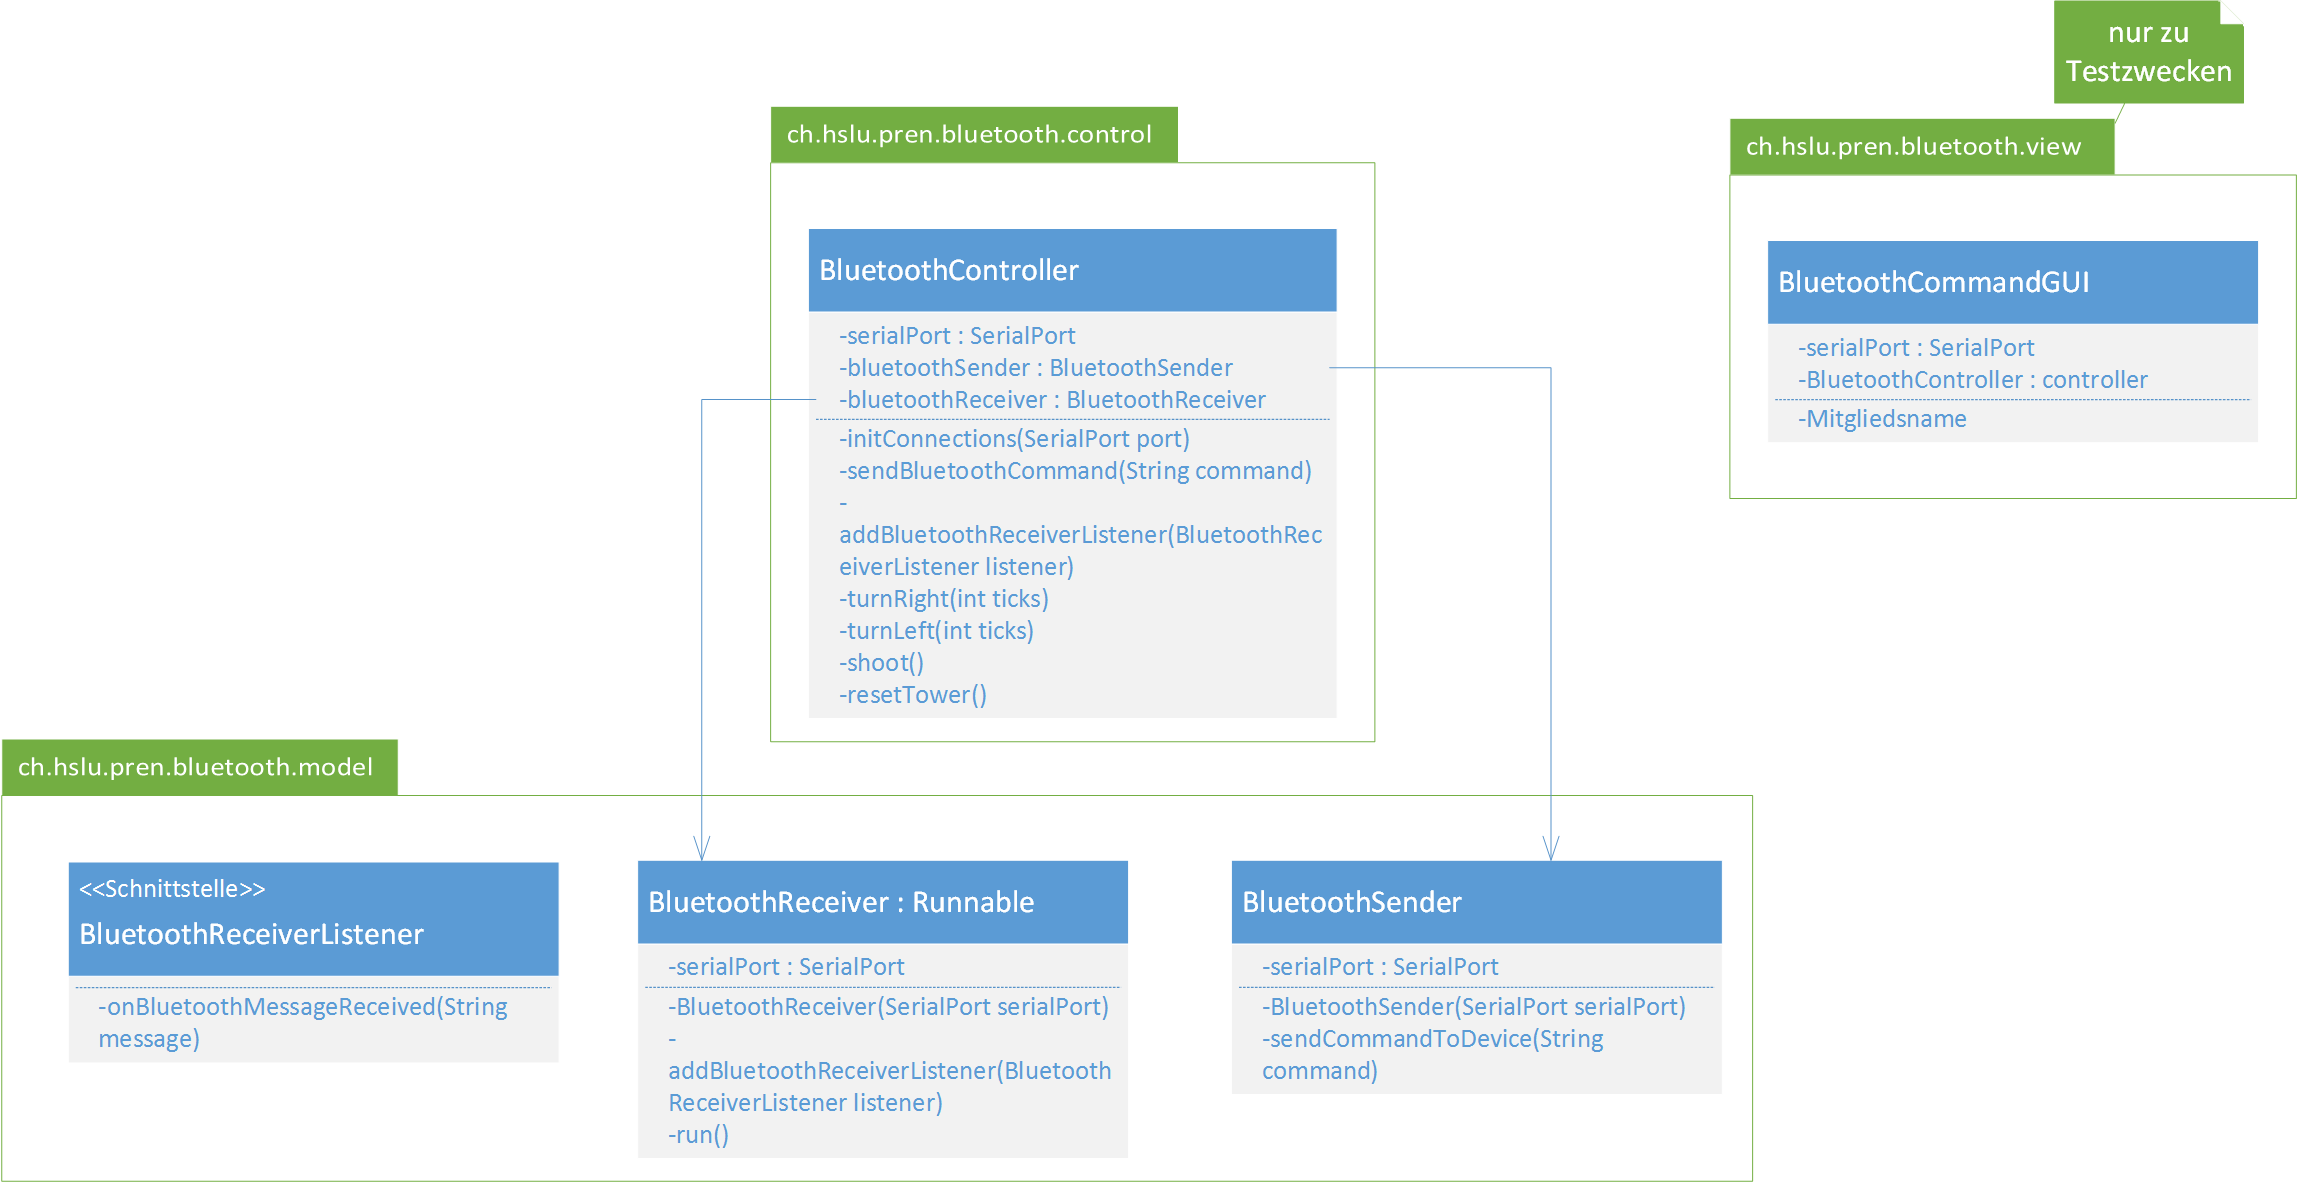
\includegraphics[width=0.9\textwidth, trim=0 10 0 0, clip=true]{../fig/Klassendiagramm_Bluetoothmodul.png}
	\caption{Klassendiagramm Bluetoothmodul}
	\label{fig:Klassendiagramm Bluetoothmodul}        
\end{figure} \\
Details zu den Methoden und den verwendeten Datentypen sind in der JavaDoc festgehalten. \\\\
\textbf{Einsatz, Abläufe, Voraussetzungen und Zusicherungen}
\begin{itemize}
	\item{Bevor Daten über die Schnittstelle ausgetauscht werden können, muss mittels \\
        \verb?initConnections(String serialPortName)? ein gültiger serieller 
        Port definiert werden. Der konfigurierte Port gilt für alle darauf 
        folgenden command-Aufrufe. }
	\item{Ein Wechsel des seriellen Ports, d.h. Umkonfigurierung mit \verb?initConnections(String serialPortName)?, ist nun jederzeit möglich.}
	\item{Eine Klasse, die das Interface \verb?BluetoothReceiverListener? implementiert, kann als Observer für empfangene Nachrichten des BluetoothReceivers fungieren.}
\end{itemize}
%\clearpage
%\noindent
\textbf{Aufbau und Konfiguration} \\
Keine zusätzlichen Informationen. \\\\
\textbf{Fehlerbehandlung} \\
Die Fehlerbehandlung wird über unchecked Exceptions realisiert. Details siehe JavaDoc. \\\\
\textbf{Beispielverwendung} \\
Der folgende Codeausschnitt zeigt die Verwendung der Schnittstelle anhand 
einer beispielhaften Implementation BluetoothController: 
\lstinputlisting[caption={Beispiel zur Verwendung des BluetoothControllers}]{../../sw/PrenManager/src/TestGUI/newClass.java}

\clearpage
\subsubsection{Spezifikation Bilderkennung}

\lstsettingjava

\begin{table}[h!]
    \centering
	\begin{zebratabular}{lllll}
        \rowcolor{gray}
		Version & Datum & Autor & Bemerkung & Status \\ 
		1.0.0 & 26.03.2015 & SN & Initiale Fassung & freigegeben \\ 
		1.0.1 & 15.04.2015 & SN & Initiale Fassung & freigegeben \\ 
		2.0.1 & 07.05.2015 & PK & Anpassung für Erkennung-Klasse & freigegeben \\ 
	\end{zebratabular} 
	\caption{Steckbrief der Klasse Erkennung}
\end{table}

\noindent
\textbf{Operationen und Datenstukturen} \\
Die Schnittstelle stellt folgende Methoden und Datentypen zur Verfügung:  \\
\begin{figure}[h!]          
	\centering             
	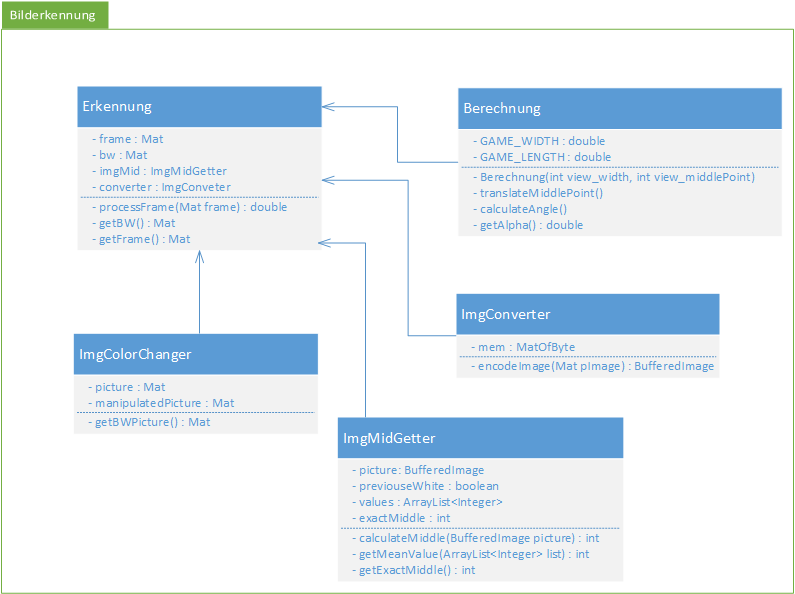
\includegraphics[width=0.8\textwidth]{fig/Klassendiagramm_Erkennung.png}
	\caption{Klassendiagramm Bilderkennung}
	\label{fig:Klassendiagramm Bilderkennung}        
\end{figure} \\
Details zu den Methoden und den verwendeten Datentypen sind in der JavaDoc festgehalten. \\

\noindent
\textbf{Einsatz, Abläufe, Voraussetzungen und Zusicherungen}
\begin{itemize}
	\item{Die Erkennung Klasse wird wie folgt initialisiert: \verb?Erkennung erkenner = new Erkennung();? }
	\item{Es gibt die Funktion \verb?processFrame(Mat frame)? mit welchem ein Bild abgearbeitet wird und den Winkel als double zurückliefert.}
\end{itemize}

\noindent
\textbf{Aufbau und Konfiguration} \\
Keine zusätzlichen Informationen. \\

\noindent
\textbf{Fehlerbehandlung} \\
Die Fehlerbehandlung wird über unchecked Exceptions realisiert. Details siehe JavaDoc. \\

\noindent
\textbf{Beispielverwendung} \\
Der folgende Codeausschnitt zeigt die Verwendung der Schnittstelle anhand einer beispielhaften Implementation BluetoothController: \\
\lstinputlisting[caption={Beispiel zur Verwendung der Bilderkennung}]{../../sw/PrenManager/src/TestGUI/Erkennung-Example.java}

\clearpage
\subsubsection{Spezifikation ImageGetter}

\lstsettingjava

\begin{table}[h!]
    \centering
	\begin{zebratabular}{lllll}
        \rowcolor{gray}
		Version & Datum & Autor & Bemerkung & Status \\ 
		1.0.0 & 30.03.2015 & KW & Initiale Fassung & freigegeben \\ 
		1.0.1 & 16.04.2015 & KW & Initiale Fassung & freigegeben \\ 
		2.0.1 & 14.05.2015 & KW & Anpassung Bilderkennung & freigegeben \\ 
	\end{zebratabular} 
	\caption{Steckbrief der Klasse ImageGetter}
\end{table}

\noindent
\textbf{Operationen und Datenstukturen} \\
Die Schnittstelle stellt folgende Methoden und Datentypen zur Verfügung:  \\
\begin{figure}[h!]          
	\centering             
	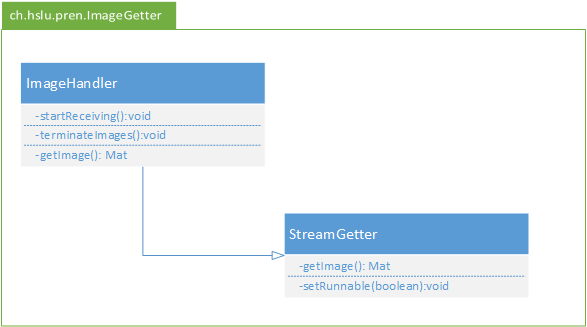
\includegraphics[width=0.7\textwidth]{../fig/Klassendiagramm_ImageGetter.png}
	\caption{Klassendiagramm ImageGetter}
	\label{fig:Klassendiagramm ImageGetter}        
\end{figure} \\
Details zu den Methoden und den verwendeten Datentypen sind in der JavaDoc festgehalten. \\

\noindent
\textbf{Einsatz, Abläufe, Voraussetzungen und Zusicherungen}
\begin{itemize}
	\item{Die ImageGetter-Klasse wird wie folgt initialisiert: 
        \verb?ImageHandler imgHandler = new ImageHandler();? }
	\item{Mittels \verb?startReceiving()? der StreamGetter-Thread gestartet 
        werden. Der StreamGetter steuert die Kamera an und speichert immer das 
        aktuellste Bild. Dieses kann vom ImageHandler mittels 
        \verb?getImage()? geholt werden. Der ImageHandler stellt dieses Bild 
        dann mit der eigenen \verb?getImage()?-Funktion als Mat-Objekt zu 
        Verfügung. Der Thread kann mittels \verb?terminateImages()? beendet 
        werden.}
\end{itemize}

\noindent
\textbf{Aufbau und Konfiguration}  \\
Keine zusätzlichen Informationen. \\

\noindent
\textbf{Fehlerbehandlung} \\
Die Fehlerbehandlung wird über unchecked Exceptions realisiert. Details siehe JavaDoc. \\

\clearpage
\noindent
\textbf{Beispielverwendung} \\
Der folgende Codeausschnitt zeigt die Verwendung der Schnittstelle anhand einer beispielhaften Implementation ImageGetter: \\
\lstinputlisting[caption={Beispiel zur Verwendung des ImageGetters}]{../../sw/PrenManager/src/TestGUI/TestImageGetter.java}
